\documentclass[a4paper, 12pt]{article}
\usepackage[a4paper,top=1.0cm, bottom=0.5cm, left=0.25cm, right=0.75cm]{geometry}
\usepackage[utf8]{inputenc}
\usepackage{mathtext}
\usepackage{amsmath}
\usepackage{amsfonts}
\usepackage[english, russian]{babel}
\usepackage{indentfirst}
\usepackage{longtable}
\usepackage{graphicx}
\graphicspath{{pictures/}}
\DeclareGraphicsExtensions{.pdf,.png,.jpg}
\usepackage{natbib}
\usepackage{mathrsfs}
\usepackage[europeanresistors, americaninductors]{circuitikz}

\title{
2.5.1 

Измерение коэффициента поверхностного натяжения жидкости.
\author{Семёнов Андрей Б02-016}
}
\date{29 апреля 2021г.}

\begin{document}
	\maketitle
	\section*{Цель работы}
		1) измерение температурной зависимости  коэффициента поверхностного натяжения дистиллированной воды с использованием известного коэффициента поверхностного натяжения спирта;  2) определение полной поверхностной энергии  и теплоты, необходимой для изотермического образования единицы  поверхности жидкости  при различной температуре.
	\section*{Оборудование}
		Прибор Ребиндера с термостатом и микроманометром, спирт и вода, стакан.
	\section*{Теория}
		Наличие поверхностного слоя приводит к различию давлений по разные стороны от искривленной границы раздела двух сред.  Для сферического пузырька с воздухом  внутри жидкости избыточное давление даётся формулой Лапласа: 
		$$\Delta P = P_{внутри} - P_{снаружи} = \frac{2 \sigma}{R}$$
		$\sigma$ - коэффициент поверхностного натяжения, $R$ - радиус кривизны поверхности раздела двух фаз. Измеряется давление $\Delta P$, необходимое для выталкивания в жидкость пузырька воздуха. 
	\section*{Экспериментальная установка}
		На рисунке ниже изображена экспериментальная установка. Исследуемая жидкость(дистиллиро- ванная вода) наливается в сосуд(колбу) В. Тестовая жидкость(этиловый спирт) наливается в сосуд Е. При измерениях колбы герметично закрываются пробками. Через одну из двух пробок проходит полая металлическая игла С. Этой пробкой закрывается сосуд, в котором проводятся измерения. Верхний конец иглы открыт в атмосферу, а нижний погружён в жидкость. Другой сосуд герметично закрывается второй пробкой. При создании достаточного разряжения воздуха в колбе с иглой пузырьки воздуха начинают пробулькивать через жидкость. Поверхностное натяжение можно определить по величине разряжения $\Delta P$, необходимого для прохождения пузырьков(при известном радиусе иглы).
		\\
		\\
		Разряжение в системе создается с помощью аспиратора А. Кран К2 разделяет две полости аспиратора. При закрытом кране К2 открывают кран К1, разряжение воздуха в колбе создаётся когда вода вытекает из крана К1 по каплям. В колбах В и С, соединённых трубками с нижней полостью аспиратора, создается такое же пониженное давление. Разность давлений в полостях с разряженным воздухом и атмосферой измеряется спиртовым микроманометром. Для стабилизации температуры исследуемой жидкости через рубашку D колбы В непрерывно прогоняется вода из термостата. 
\begin{figure}[h]
\centering
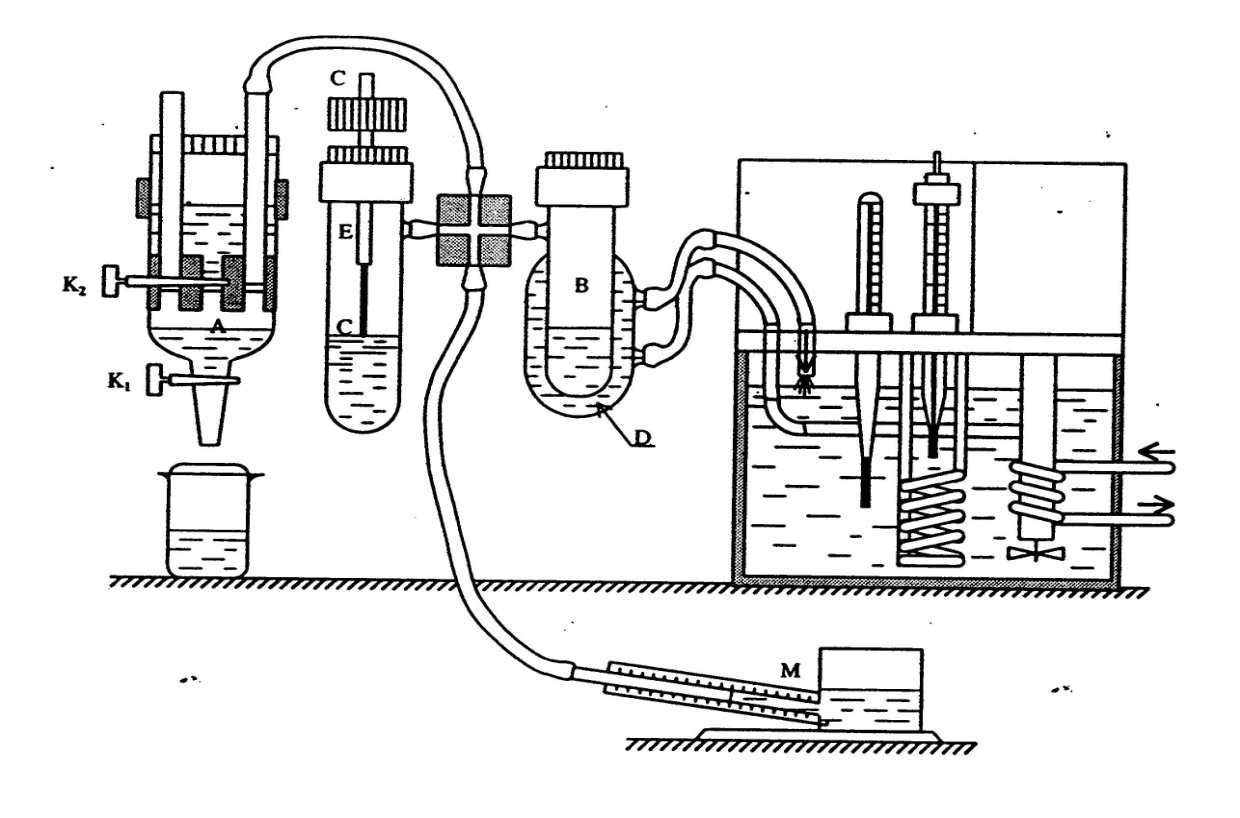
\includegraphics[width=0.7\linewidth]{Scheme}
\label{fig:scheme}			
\end{figure}
		\\
		\\
		Обычно кончик иглы лишь касается поверхности жидкости, чтобы исключить влияние гидростатического давления столба жидкости. Однако при измерении температурной зависимости коэффициента поверхностного натяжения возникает ряд сложностей. Во-первых, большая теплопроводность металлической трубки приводит к тому, что температура на конце трубки заметно ниже, чем в глубине жидкости. Во-вторых, тепловое расширение поднимает уровень жидкости при увеличении температуры.
		\\
		\\
		Обе погрешности можно устранить, погрузив кончик трубки глубже в жидкость. Полное давление, измеренное при этом микроманометром, $P = \Delta P + \rho gh$. $\rho gh$ не зависит от температуры жидкости. Величину $\rho gh$ следует измерить двумя способами. Во-первых, замерить величину $Р1= \Delta P'$, когда кончик трубки только касается поверхности жидкости. Затем при этой же температуре опустить иглу глубже в жидкость и замерить $Р2 = \rho gh + \Delta P"$ ($\Delta P'$, $\Delta P"$ – давление Лапласа). Из-за несжимаемости жидкости можно положить $\Delta P'= \Delta P"$ и тогда $\rho gh = Р2 - Р1$. Во-вторых, при измерениях Р1 и Р2 замерить линейкой глубину погружения иглы h.

\section{Выполнение работы}

Измеряем максимальное давление $\Delta P_{alcohol}$  при  пробулькивании пузырьков воздуха через спирт. Записываем все в таблицу. Измеряем диаметр иглы по микроскопу, так же записываем в таблицу. Измеряем диаметр, полученный при измерении разности давлений спирта по формуле $d = \dfrac{4 \sigma}{\Delta P}$ , $\sigma = 0.02266 N/m $
\\$\sigma_{\Delta P} = \sqrt{\frac{\sum\limits_{i=1}^n(\Delta P_i - P_{average})^2}{n(n-1)}} $

\begin{tabular}{|c|c|c|c|}
\hline
$\Delta P$, Па              & $\sigma_{\Delta P}$, Па              & $d$, мм              & $\sigma_{d}$, мм              \\ \hline
82,4                        & 0.93                                    & 1,10                 & 0,12                          \\ \hline
80,1                        & 0.93                                    & 1,13                 & 0,12                          \\ \hline
84,7                        & 0.93                                    & 1,07                 & 0,12                          \\ \hline
82,4                        & 0.93                                    & 1,10                 & 0,12                          \\ \hline
\multicolumn{4}{|c|}{ $\overline{d_{alcohol}} = (1,1 \pm 0,12)$ мм, $d_{microscope} = (1,1 \pm 0,05)$ мм} \\ \hline
\end{tabular}

Измеряем при комнатной температуре $h_1$ и $h_2$ относительно какой-нибудь неподвижной детали, и измеряем $P_{1max}$ и $P_{2max}$ по $\Delta P$ найдем $\Delta h$ и сравним с $h_1 - h_2$. Учитываем, что при подсчете мы измеряем с помощью монометра $P = \Delta P + \rho g \Delta h$. Записываем результаты в таблицу. \\$\sigma_{P_1} = 2.26$ \\$\sigma_{P_2} = 1.03$ \\$\sigma_{\Delta h} = \sqrt{\sigma_{P_1}^2 + \sigma_{P_2}^2 } = 2.48$
\begin{center}
\begin{tabular}{|c|c|c|c|}
\hline
$P_1$, Па             & $h_1$, см            & $P_2$, Па            & $h_2$, см            \\ \hline
274                   & 1,8                  & 363                  & 0,8                  \\ \hline
274,7                 & 1,8                  & 360                  & 0,8                  \\ \hline
273,3                 & 1,8                  & 365                  & 0,8                  \\ \hline
265                   & 1,8                  & 363                  & 0,8                  \\ \hline \hline
271,75                & 1,8                  & 362,75               & 0,8                  \\ \hline
\multicolumn{4}{|c|}{$h_1 - h_2 = 1$ см, $\dfrac{P_2 - P_1}{\rho g} = (0,93 \pm 0,24)$ см} \\ \hline
\multicolumn{4}{|c|}{$\rho g \Delta h = (91 \pm 2,66)$ Па}                                  \\ \hline
\end{tabular} \\
\begin{tabular}{|c|c|c|c|c|c|}
\hline
$T$, K & $P$, Па & $\sigma_P$, Па & $\Delta P$, Па & $\sigma_{water} \cdot 10^{-3}$, Н/м & $\sigma_{\sigma_{water}} \cdot 10^{-3}$, Н/м \\ \hline
25,00  & 364,00  & 2.14           & 273,00    & 75,08                               & 0,61                                        \\ \hline
30,00  & 362,00  & 2.14           & 271,00    & 74,53                               & 0,61                                        \\ \hline
35,00  & 359,00  & 2.14           & 268,00    & 73,70                               & 0,61                                        \\ \hline
40,00  & 357,00  & 2.14           & 266,00    & 73,15                               & 0,61                                        \\ \hline
45,00  & 353,00  & 2.14           & 262,00    & 72,05                               & 0,61                                        \\ \hline
50,00  & 350,00  & 2.14           & 259,00    & 71,23                               & 0,61                                       \\ \hline
55,00  & 347,00  & 2.14           & 256,00    & 70,40                               & 0,61                                       \\ \hline
60,00  & 343,00  & 2.14           & 252,00    & 69,30                               & 0,61                                       \\ \hline
50,00  & 345,00  & 2.14           & 254,00    & 69,85                               & 0,61                                       \\ \hline
45,00  & 347,00  & 2.14           & 256,00    & 70,40                               & 0,61                                       \\ \hline
30,00  & 350,00  & 2.14           & 259,00    & 71,23                               & 0,61                                        \\ \hline
\end{tabular}
\\
Представляем данные в виде графика и находим $\dfrac{d \sigma}{dT}$

\begin{minipage}[h]{0.69\textwidth}
\begin{tikzpicture}[scale = 1]
\begin{axis}[
    axis lines = left,
    legend style={at={(0.9, 0.3)}},
    xlabel = {$T$, $C$},
    ylabel = {$\sigma 10^{-3}$, $N/m$},
    xmin=20 , xmax=70,
    ymin=60 , ymax=75,
	ymajorgrids = true,
	xmajorgrids = true
]
\addplot[
	mark = square, 
	mark options = {
		scale = 1.5, 
		fill = red, 
	},
	ymajorgrids = true,
	xmajorgrids = true,
	color = blue 
]  coordinates {
	(25, 75.08) (30, 74.53) (35, 73.70) (40, 73.15) (45, 72.05) (50, 71.23) (55, 70.40) (60, 69.30)};

\addplot [
    domain=0:100, 
    samples=1000, 
    color=red,
]
{-x*0.16+79.13};

\legend{ 
	Experiment,
	Theory
};
\end{axis}
\end{tikzpicture}
\end{minipage}


C помощью МНК определим значение коэффициента угла наклона данного графика:

$ k = \frac{<\sigma T>-<\sigma><T>}{<T^2>-<\sigma>^2} =-0.16 $;
\\$ a = <\sigma> - k<T> = 79.13 $
$\sigma_{k} = \frac{1}{\sqrt{n}}\sqrt{\frac{<\sigma^2> - <\sigma>^2}{<T^2> - <T>^2}-k^2} = 0.01$

$q = -T\frac{d\sigma}{dT}$
\begin{minipage}[h]{0.69\textwidth}
\begin{tikzpicture}[scale = 1]
\begin{axis}[
    axis lines = left,
    legend style={at={(0.9, 0.3)}},
    xlabel = {$T$, $K$},
    ylabel = {$q$, $Dj$},
    xmin=0 , xmax=100,
    ymin=0 , ymax=10,
	ymajorgrids = true,
	xmajorgrids = true
]

\addplot [
    domain=0:100, 
    samples=1000, 
    color=red,
]
{0.016*x};

\legend{ 
	q(T)
};
\end{axis}
\end{tikzpicture}
\end{minipage}

\section{Результаты}

\begin{enumerate}
	\item Диаметр полученный нами в результате измерения разности давлений спирта совпал с измеренным под микроскопом значением.
	\item Экспериментальное значение глубины погружения иглы отклонилось от истинного на 7%.
	\item $\dfrac{d \sigma}{dT}$ отклонился от $\dfrac{d \sigma_t}{dT}$ на 0.06. 

\end{enumerate}
\end{document}		
